\todo{finish this and use the sections as a guide}

\subsection{Context}
The UAV Challenge \cite{ref:challenge}, organised by the Queensland University of Technology and the CSIRO, is a biennial competition that aims to push the boundaries of current autonomous aircraft technology. The 2016 challenge is titled ``Medical Express'', and charges teams with solving the issues raised above.\\

Competitors must develop an aircraft that can fly to a known area (up to 30km away) through specific transit corridors, search for and correctly identify ``Outback Joe'', land close to him in an obstacle-rich environment, accept a pre-prepared blood sample, and then fly back to base. All of these actions must be completed within one hour, and must be fully autonomous; that is, after receiving the ``start'' signal the aircraft must have no human input.

\subsection{Project Outline}
This project involves the development of an autonomous Unmanned Aerial Vehicle (UAV) with the capabilities to compete in the 2016 UAV Challenge. Given the Challenge specifications above, a number of design and performance requirements were identified that aircraft must meet in order to be successful:
\begin{enumerate}[label=\bfseries R\arabic*:] \itemsep-2pt
	\item Aircraft must be autonomous
	\item Take-off and landing in obstacle-rich environments (i.e. without a runway)
	\item Total flight endurance of at least 60km
	\item Total flight duration of up to 60 minutes
	\item Automated in-flight identification of a known target
	\item Ability to receive 500g payload upon landing
\end{enumerate}

It is anticipated that there will be several Capstone student teams continuing development of the UAV in 2016. Given the requirements listed above, and the timeline of the Challenge, the \ID project team sought to develop a working prototype with which to achieve the basic functionality required to compete in the Challenge. As such, the following objectives were selected for the project:
\begin{enumerate}[label=\bfseries O\arabic*:] \itemsep-2pt
	\item Register for the 2016 UAV Challenge
	\item Development of a prototype UAV for future teams to build on
	\item Development of autonomous flight controls to achieve \textbf{R1}
	\item Development of a novel hybrid flight system, incorporating both Vertical Take-Off and Landing (VTOL) and Fixed-Wing flight modes, for future teams to build upon to achieve requirements \textbf{R2}, \textbf{R3} and \textbf{R4}
	\item Development of in-flight search and obstacle avoidance mechanisms to be able to achieve \textbf{R5}
\end{enumerate}

The remaining sections of the report will discuss the work conducted by \ID in developing a working prototype for the UAV Challenge, beginning with a brief review of existing approaches that motivated the design of the UAV developed in this project. The following sections will discuss the various development domains of the UAV, including its design, flight and planning systems, and sensing systems, with a particular focus on the novel transition system developed for hybrid flight.

\subsection{Mission Breakdown}
\label{sec:flightmaneuvers}
The Medical Express mission can be broken down into three distinct flight maneuvers:
\begin{enumerate}[label=\bfseries M\arabic*:] \itemsep-2pt
	\item Hover flight, including vertical take-off to cruising height, and landing
	\item Fixed-wing flight, navigating through waypoints and keeping within GeoFence boundaries
	\item Aerial search
\end{enumerate}

Using these maneuvers, completing the mission can be described as completing the sequence of actions\\
\begin{tabular}{r l l}
	1. & Mission start after being armed & (\textbf{M1}) \\ 
	2. & Navigate to Joe's location & (\textbf{M2}) \\ 
	3. & Aerial search to identify Joe & (\textbf{M3}) \\ 
	4. & Land near Joe to collect blood & (\textbf{M1}) \\ 
	5. & Take-off after being re-armed & (\textbf{M1}) \\ 
	6. & Navigate back to base & (\textbf{M2}) \\ 
	7. & Land at base & (\textbf{M1}) \\ 
\end{tabular}\\

Executing this mission on a purely fixed-wing or rotor-based aircraft is unlikely to be successful; instead, teams will need to design an aircraft that makes use of both flight modes.

\subsection{Proposed Design}
The initial prototype design for this project will use a PixHawk flight controller in a Skywalker X8 airframe, mounted with three motors in a tri-coptor configuration. The aircraft will also be fitted with a transition system, to rotate the front motors and enable the aircraft to fly in both VTOL and fixed-wing modes. Finally, the aircraft will be mounted with various sensors, discussed in Section \ref{sec:sensing}, including a camera and LiDAR, to provide sensing capabilities for planning, obstacle detection and autonomous flight.\\

Figure \ref{fig:hardwarearch-exec} shows a high level overview of the hardware architecture planned for the current and future teams.

\begin{figure}[!h]
	\centering
	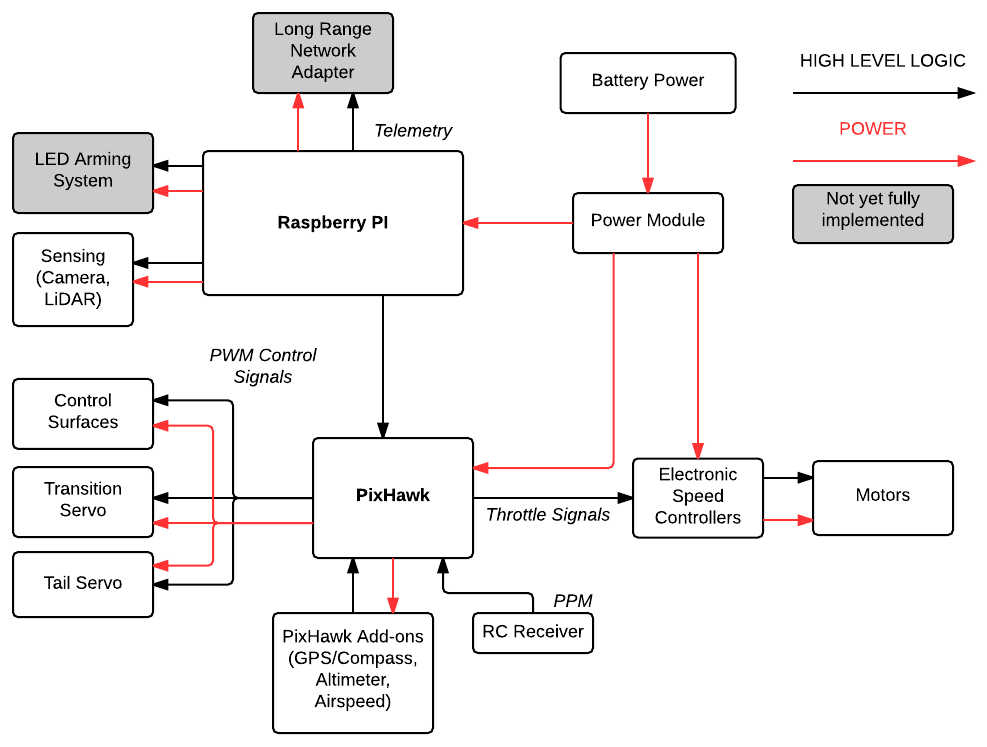
\includegraphics[width=380pt]{\IMAGEPATH /Diagrams/hardware}
	\caption{High level hardware architecture}
	\label{fig:hardwarearch-exec}
\end{figure}

\subsection{Why Transition?}
In order for the UAV to complete the objectives listed previously, it must be capable of both long range flight and vertical take-off and landing. Implementing a transition system, rather than fit the UAV with both fixed-wing and VTOL flight systems, allows it to achieve this capability while also being lighter, and more aerodynamic. The transition systems is the foundation for achieving the range and endurance requirements of the UAV Challenge.

\subsection{Software Development}
Any aircraft participating in the UAV Challenge must be autonomous, only interacting with a human to be armed or disarmed at the beginning and end of the mission. A framework for autonomous flight was developed in Python for the Raspberry Pi, based on the following considerations:
\begin{itemize}
	\item \textbf{Extendibility:} Software is designed so that future teams can easily add functionality to the autonomous systems
	\item \textbf{Concurrency:} Software launches several parallel processes, enabling real-time interaction between the many subsystems of the aircraft and software
	\item \textbf{Low-Latency:} All processes must have little to no delay in communication, allowing for real-time operation 
\end{itemize}

Figure \ref{fig:softwarearchitecture-exec} shows the software architecture for the autonomous flight and intelligence systems implemented on the Raspberry Pi, consisting of a number of parallel processes, two objects to monitor the state of the aircraft, and objects to facilitate inter-process communication. Each process shown in Figure \ref{fig:softwarearchitecture-exec} performs a specific function:
\begin{itemize}
	\item \textbf{Autopilot:} Acts as an interface to pass flight commands from the UAV software to the PixHawk, and to monitor and respond to sensor data
	\item \textbf{Flight:} Generates the desired flight path for the aircraft, and sends flight commands to the Autopilot process
	\item \textbf{UAVStateUpdater:} Monitors and updates the state of the aircraft by interfacing with internal sensors, including GPS, accelerometer, etc; manages the UAVState object that stores sensor data
	\item \textbf{WorldStateUpdater:} Monitors and updates the state of the world by interfacing with external sensors, including camera, LiDAR and ultrasonic; manages the WorldState object that stores sensor data
	\item \textbf{BaseCommunications:} Provides a real-time data link between the aircraft and the ground station
	\item \textbf{Logging:} Retrieves data from other modules and generates flight logs for reviewing mission performance
\end{itemize}

\begin{figure}[!ht]
	\centering
	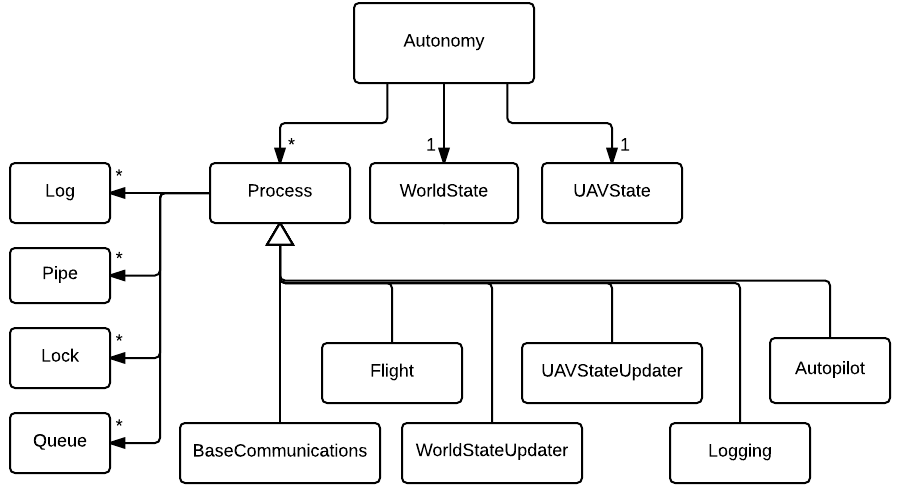
\includegraphics[width=340pt]{\IMAGEPATH /Diagrams/software}
	\caption{High level software architecture}
	\label{fig:softwarearchitecture-exec}
\end{figure}

Figure \ref{fig:softwareinteraction-exec} shows the communication paths between the various processes. As a result of the multiprocessing framework, communication between modules is not as simple as passing variables through functions. Instead, whenever two or more processes communicate with each other, a dedicated ``link'' needs to be created between them. Pipes (blue in Figure \ref{fig:softwareinteraction-exec}) allow for bidirectional communication between processes, such as between the Flight and Autopilot. Queues (green in Figure \ref{fig:softwareinteraction-exec}) only allow unidirectional communication, such as between all processes and the Log process, which only needs to receive information.\\

One of the biggest dangers in parallel processing communication is data corruption or loss; one process attempts to read data from a link while another is modifying it or writing to it, resulting in the data becoming unusable. To prevent this, each process that connects with either a pipe or queue is provided with read and write ``locks''. When activated, the lock will prevent other processes from reading from, or writing to, the communication link before the current process has completed its operation.

\begin{figure}[H]
	\centering
	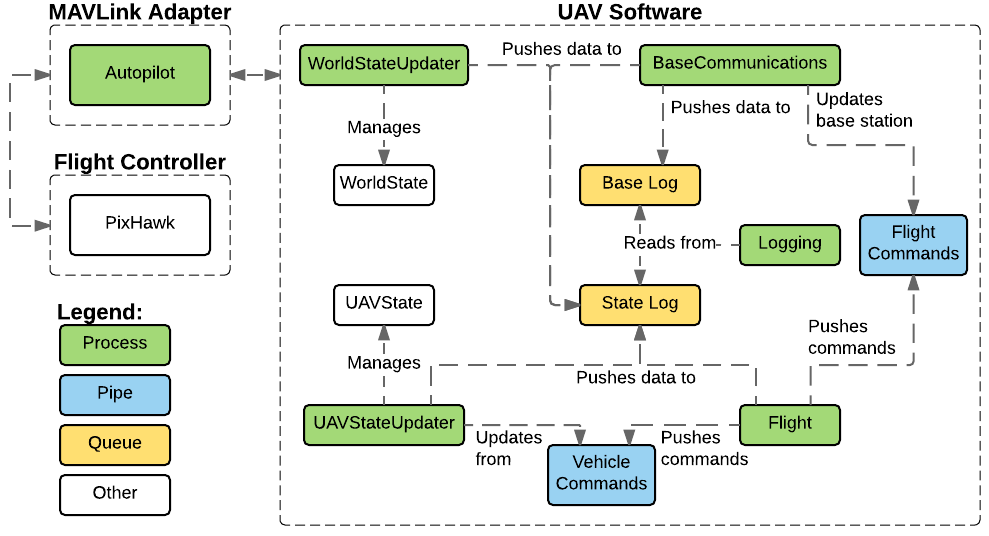
\includegraphics[width=380pt]{\IMAGEPATH /Diagrams/interaction}
	\caption{Interaction between software modules}
	\label{fig:softwareinteraction-exec}
\end{figure}

\subsection{Sensing}

Figure \ref{fig:sensing-exec} outlines the on-board sensing capabilities that are available to the aircraft. The sections below detail the motivation and use of each sensor, and are separated according to the different stages of the UAV Challenge's mission, as introduced in Section \ref{sec:flightmaneuvers}. At the time of writing, only some of the sensors mentioned below have been physically mounted to the aircraft, but each sensor's position on the aircraft has been incorporated into the aircraft's design.

\begin{figure}[!ht]
	\centering
	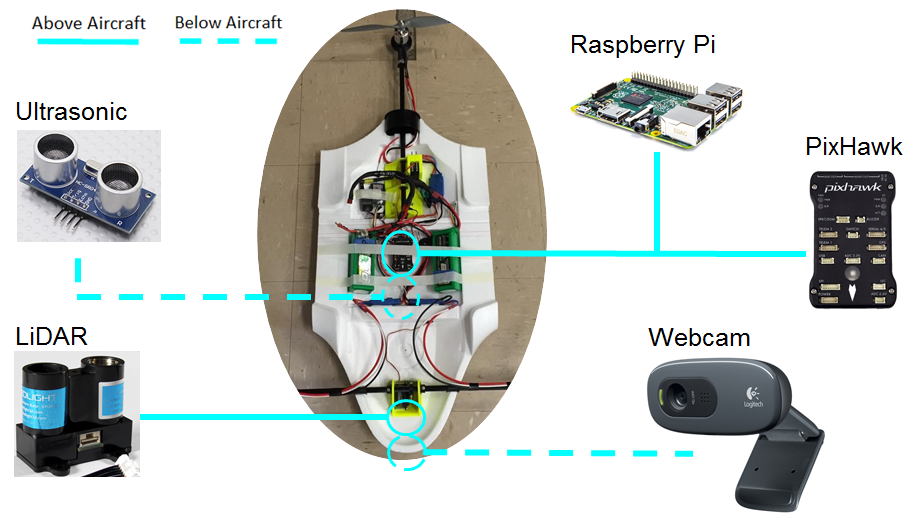
\includegraphics[width=300pt]{\IMAGEPATH /Diagrams/sensors}
	\caption{Onboard sensing capabilities, and mounting location, for Prototype \#2}
	\label{fig:sensing-exec}
\end{figure}


\subsection{Achievements, conclusion and recommendations}